\section{Models}

% \subsection{User stories}
% 
% As a user, want to get some Information from skyserver to analyze the database
% of this server and want to know, how many 
% user or client that used this server from 
% wich Countries and in wich time (Month and Year) . 
% 
% To analyze this Information in best way, i would like
%  to get Visualizing and Statistically of these Information.
% That's mean, i can get some diagram with axises like histogram.
% 
% Steps to descrip how can a normal user use this Application:
% 
% \renewcommand{\theenumi}{\arabic{enumi}}
% \renewcommand{\labelenumi}{\theenumi}
% 
% \begin{enumerate}
% 
% \item Start internet browser
% 
% \item Vist www.say pse10-analyzer.edu web page
% 
% \item 
% 
% \end{enumerate}



\subsection{Overview}\label{overview}
This picture describes the general concept of WHAT.
\begin{center}
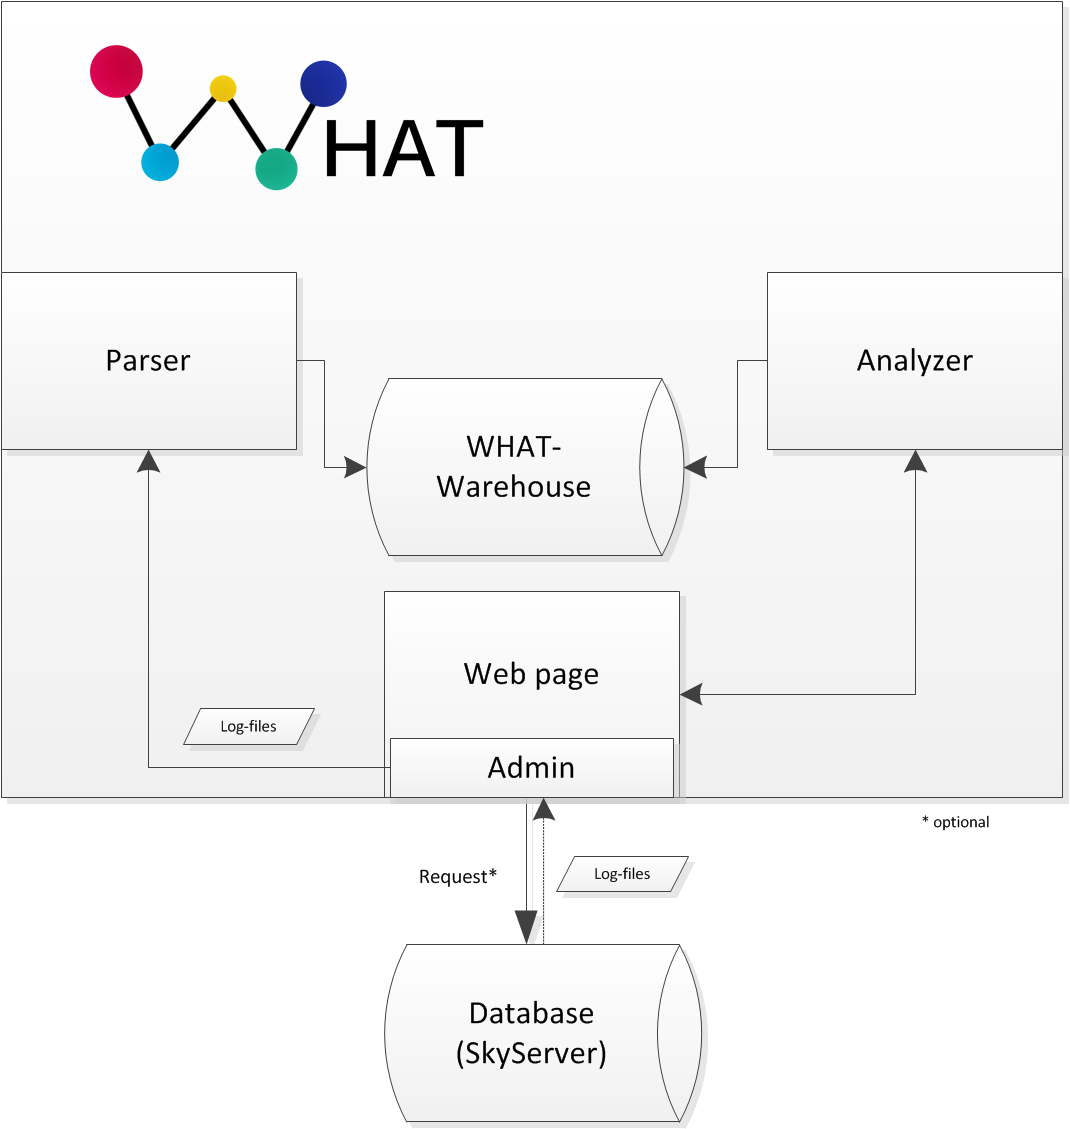
\includegraphics[width=1\linewidth]{Pictures/GenerellConcept.png}
\end{center} 
% 
% \subsubsection{Parser}
% Parser blabla
% \subsubsection{Analyzer}
% analyzer blabla
% \subsubsection{Web page}
% web page blabla


\subsection{Dynamic models}
\begin{center}
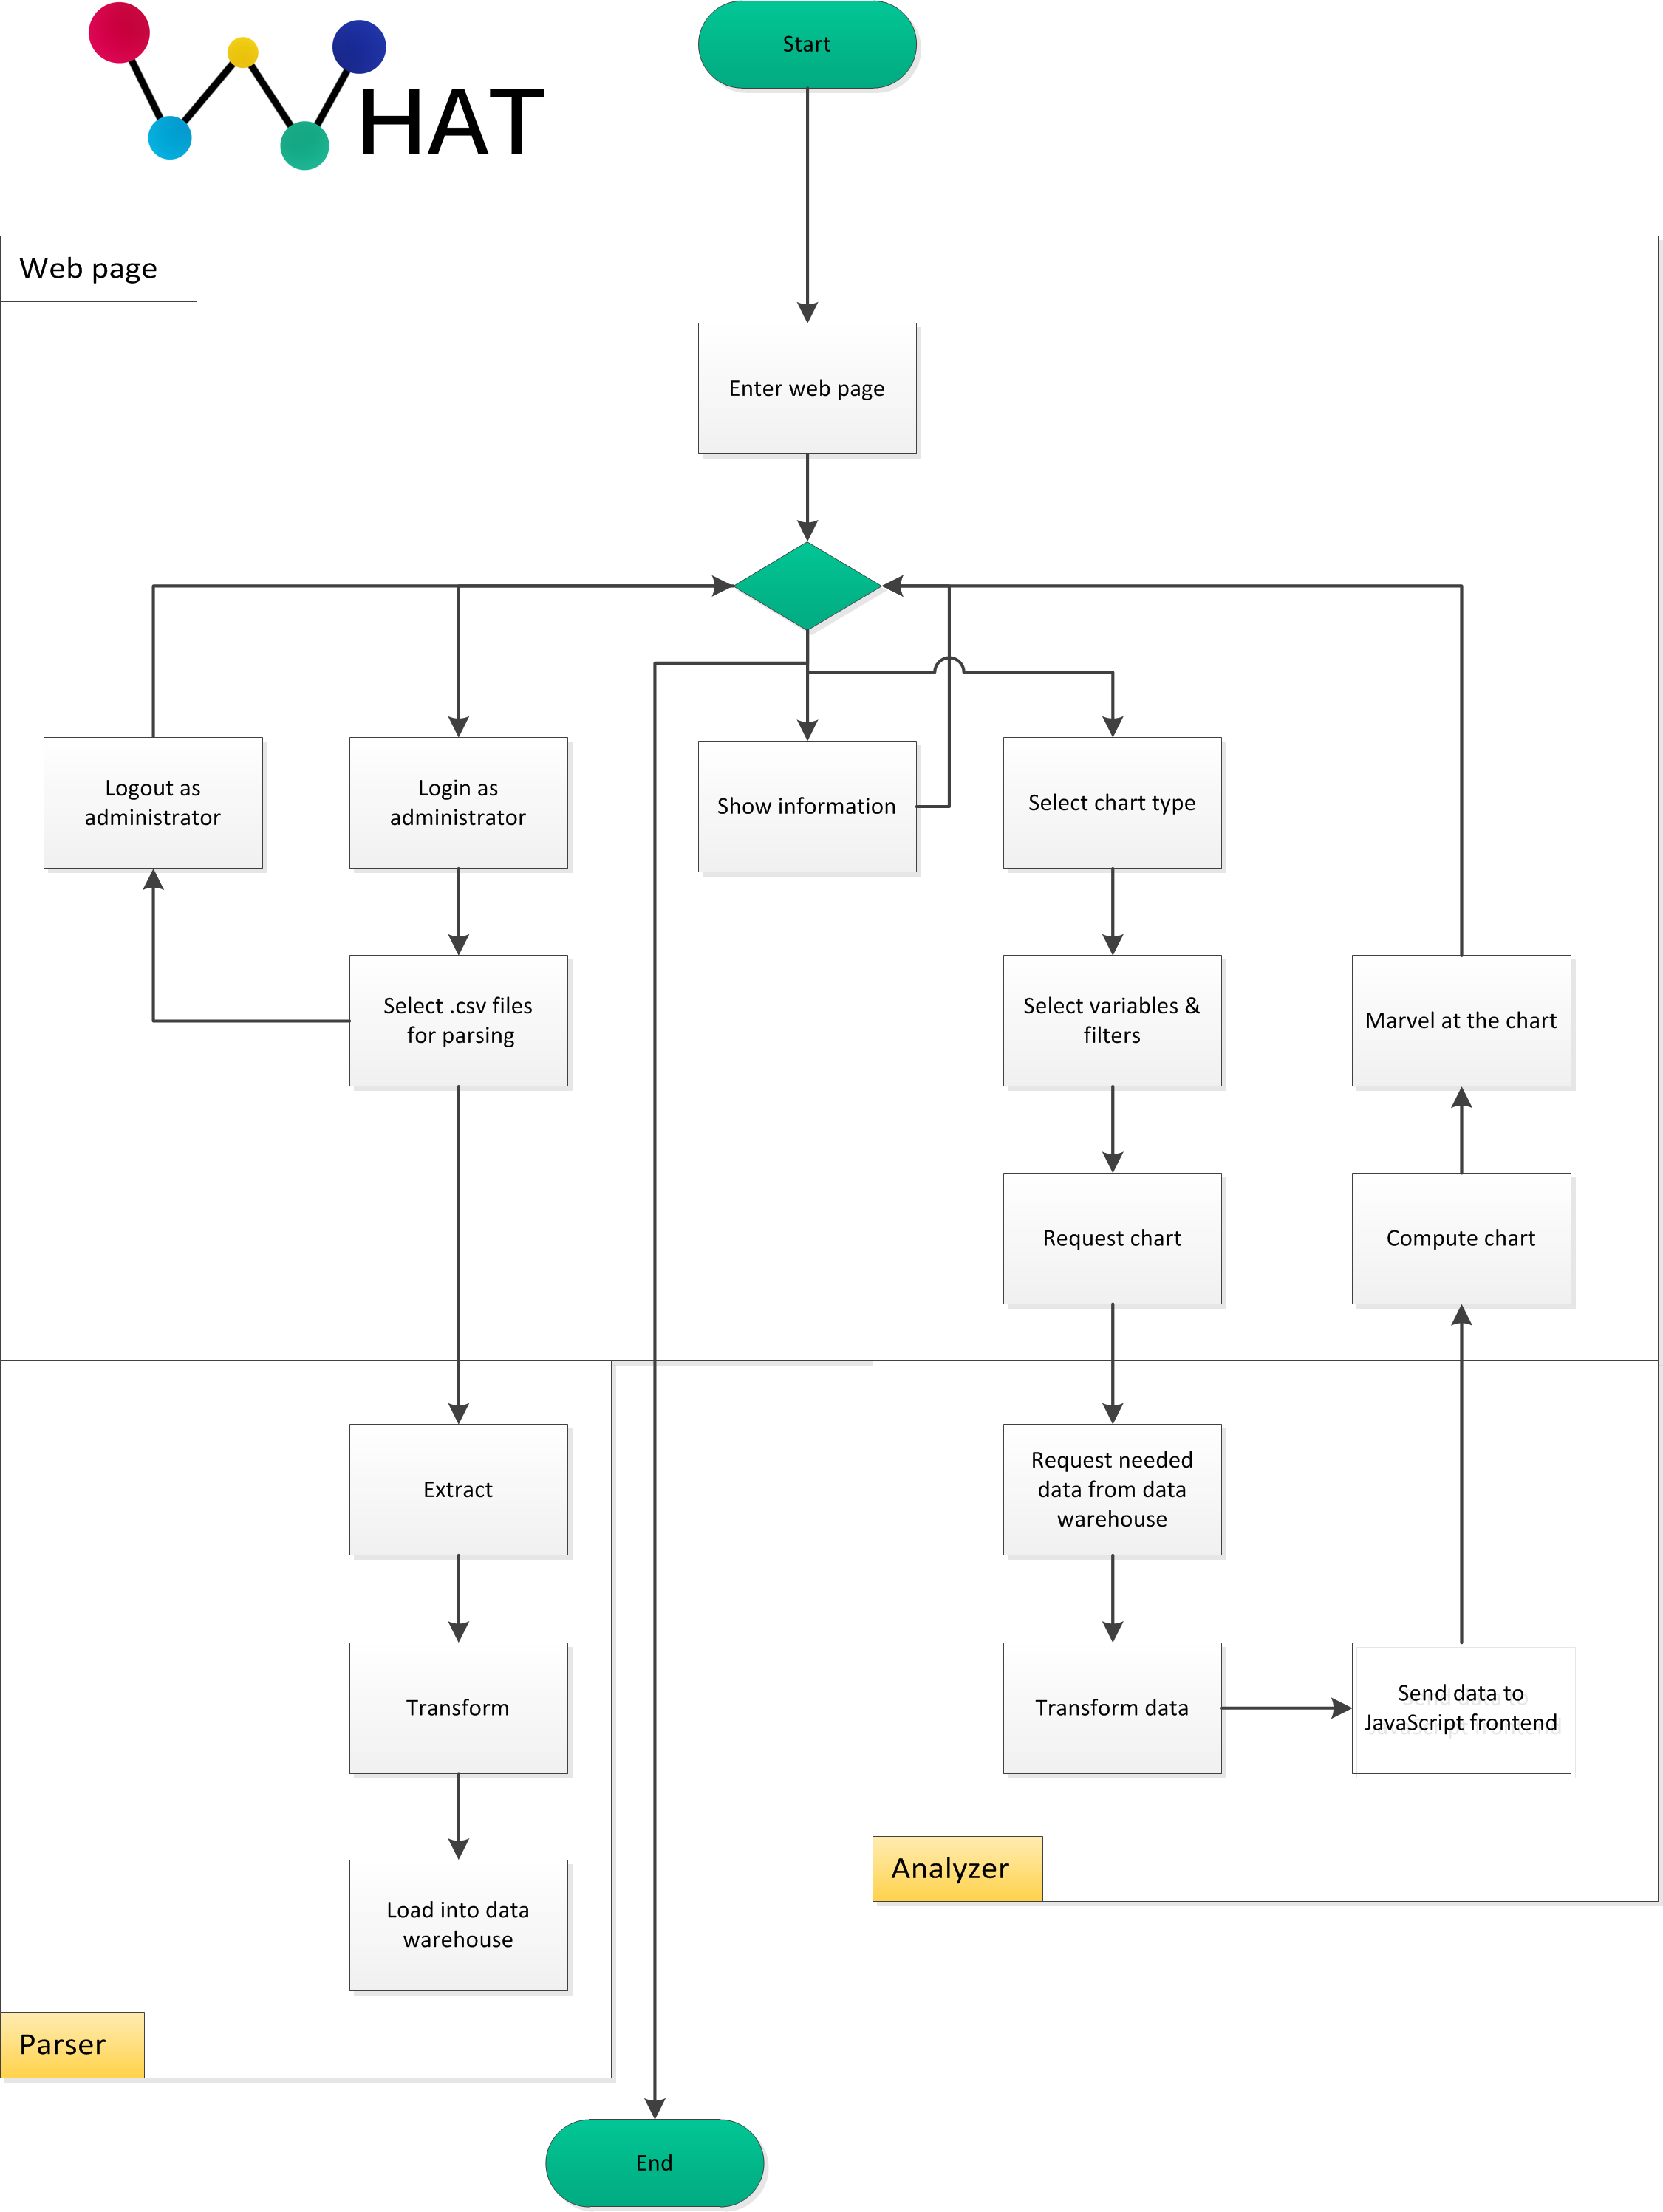
\includegraphics[width=0.85\linewidth]{Pictures/Flow1.png}
\end{center} 

\newpage
\subsection{Web interfaces}
The start page of the web page.
\begin{center}
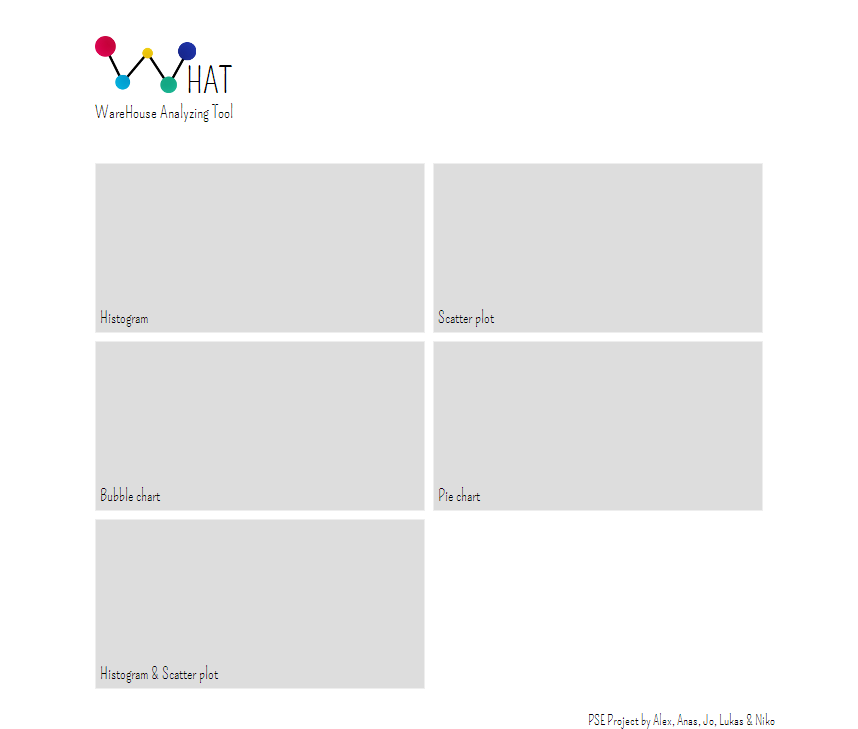
\includegraphics[width=1\linewidth]{Pictures/WHAT-Start.png}
\end{center} 
\newpage
An example for a \gls{diagram} page.
\begin{center}
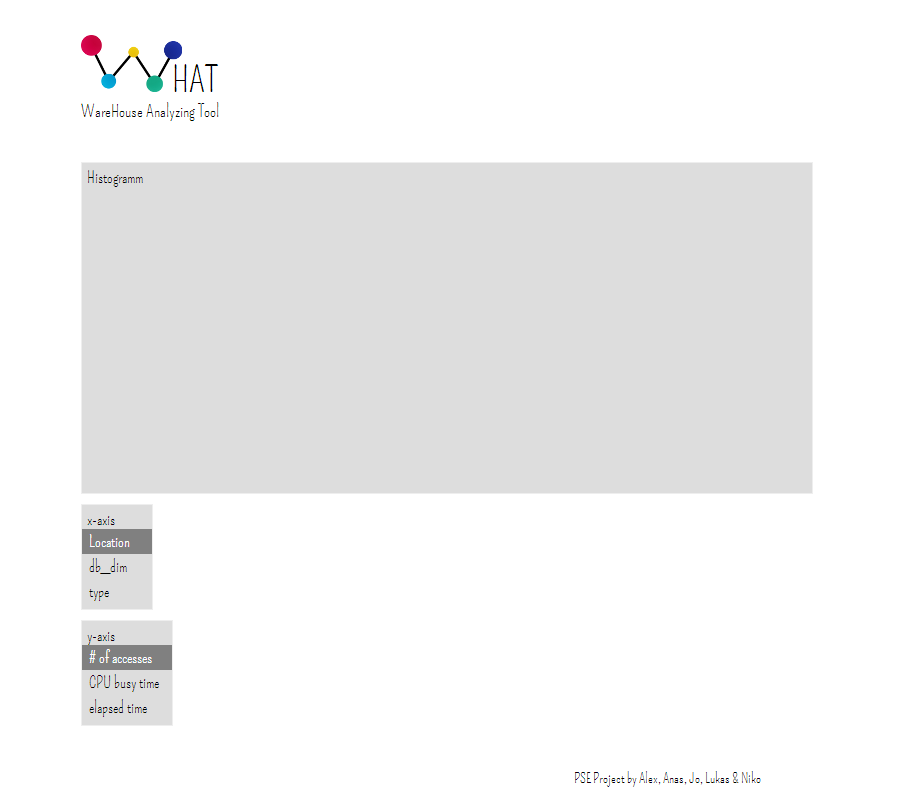
\includegraphics[width=1\linewidth]{Pictures/WHAT-Histogram.png}
\end{center} 










% \subsection{Warehouse schema}
% The warehouse may use a star schema.
% \begin{center}
% 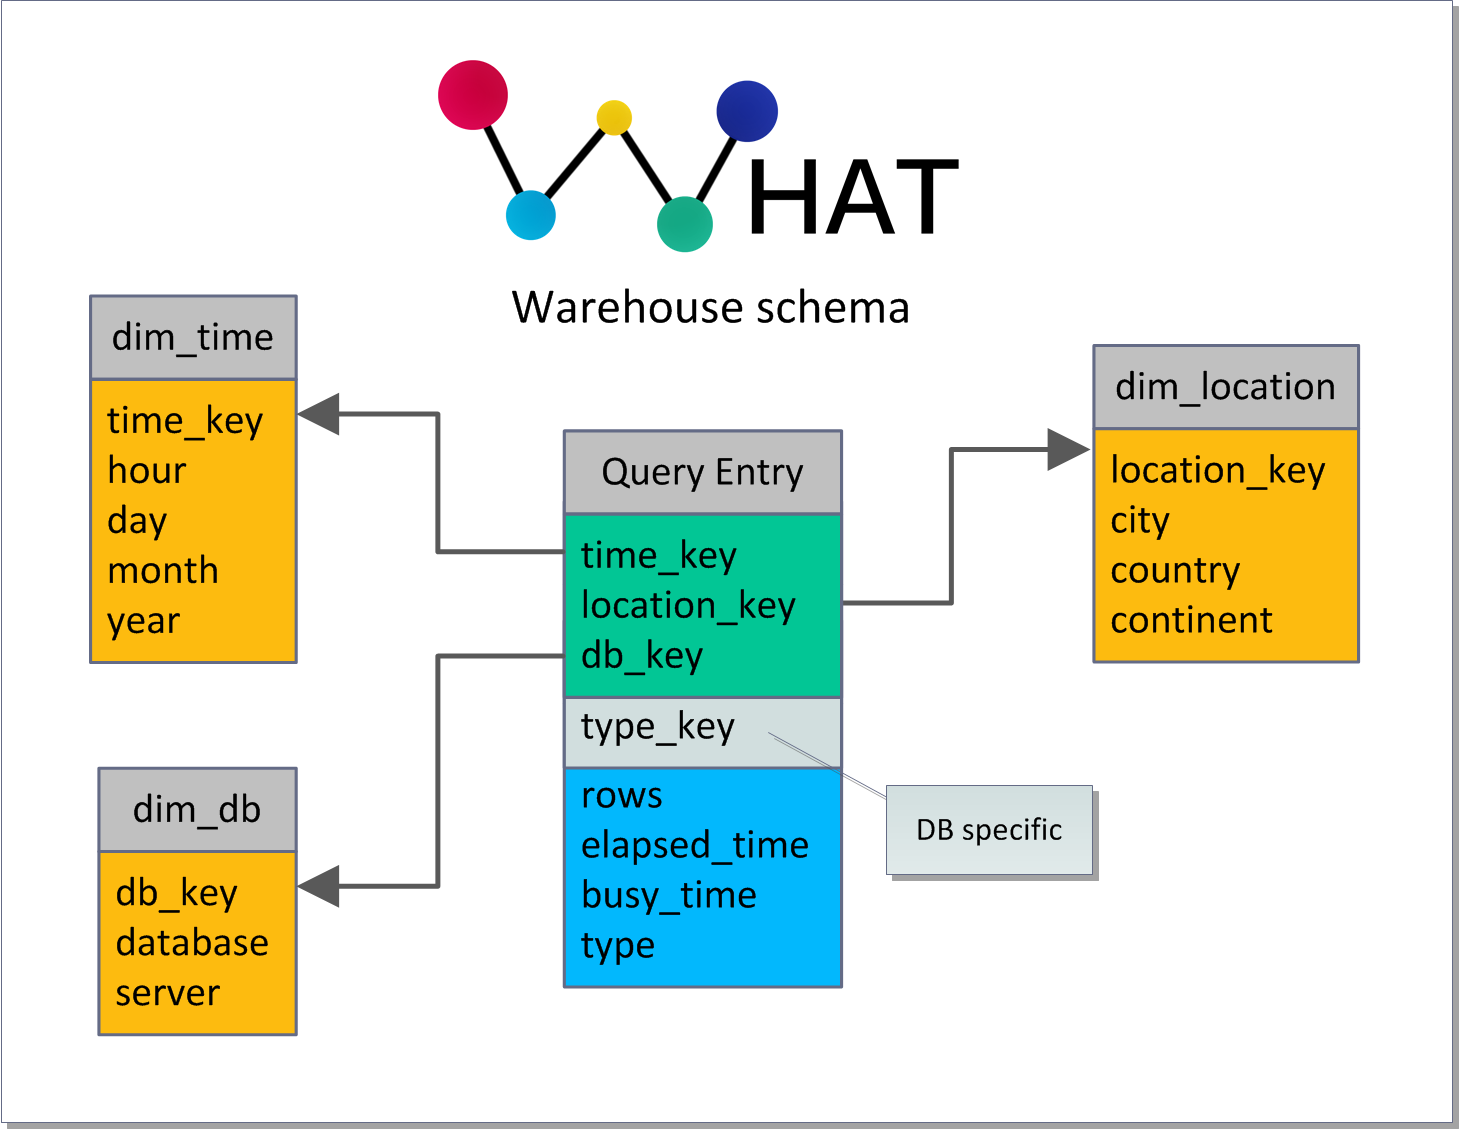
\includegraphics[width=1\linewidth]{Pictures/WareHouseSchema.png}
% \end{center}   